% !TeX root = ../main-english.tex
% !TeX spellcheck = en-US
% !TeX encoding = utf8
% -*- coding:utf-8 mod:LaTeX -*-

%This smart spell only works if no changes have been made to the chapter
%using the options proposed in preambel/chapterheads.tex.
\setchapterpreamble[u]{%
	\dictum[Carole Goble]{Better Software, Better Research}
}

\chapter{Improving scientific practice through software usability: The DataLad Handbook}
\label{chap:k2}

As outlined in the Introduction, software tools for \gls{rdm} exist.
However, their mere existence is insufficient to ensure uptake and use according to best practices.
To improve scientific practice, software tools need to empower their users through usability and documentation.
This makes documentation a major factor in the success of scientific software, and an integral part of the software development process.
This next chapter details how a documentation project for DataLad increased software quality, software popularity and enabled users to tackle complex \gls{rdm} use cases.
It refers to our original publication \citet{wagner2020datalad}.

\section{Documentation deficits of scientific software and their consequences}

Software documentation is ...

Scientific software often lacks comprehensive documentation \citet{segal2007some}.
Commonly reported reasons for this are a lack of funding, incentives, and interest by software developers (CITATION NEEDED).

Although it is commonly regarded as separate from the actual piece of software, software documentation is heavily tied to the quality of a software tool.
\citet{Parnas2011} describes a vicious circle that sets in when the quality of software documentation is poor:

\begin{quote}
\begin{enumerate}
\item Reduced [documentation] quality leads to reduced [software] usage.
\item Reduced [software] usage leads to reductions in both resources and motivation.
\item Reduced resources and motivation degrade [software] quality further
\end{enumerate}
\end{quote}


According to \citet{Parnas2011}, documentation can be categorized for use either as a \textit{tutorial} or as a \textit{reference work}.
Both kinds are needed for different audiences: Whereas experienced users and contributors need reference documents to guide further development, new users and contributors need a basic understanding of the software tool and its intended use cases.
Reference documentation can thus be suboptimal for novices: It may be incomplete, narrowly focused on individual commands, or assume existing knowledge novices lack (Segal, 2007; Pawlik et al., 2015), and can thereby discourage potential users or inhibit the adoption of valuable tools.
In an analysis of user questions in support forums of scientific software packages, \citet{swarts2019open} found that the focus in 80\% of inquiries was on operations and tasks, such as a required sequence of operations to achieve a specific goal.
In breaking down user questions by purpose, \citet{swarts2019open} further found that users were most interested in a description of operations or tasks, followed by insights about the reasons behind the action.
And in separating documentation types into ``feature-based'' (closer related to the concept of reference documentation) or ``task-based'' (closer related to the concept of a tutorial),  \citet{swarts2019open} reports twice as many questions seeking explanations in software with feature-based compared to task-based documentation.
This hints at a disconnect between knowing \textit{how} something should be done and \textit{why} it should be done this way.
These results highlight that users of scientific software show a clear need beyond the documentation of individual commands, but seek to understand general usage principles and master complex combinations of features to achieve specified goals.
This type of empowerment is what the DataLad handbook project aimed to achieve.


The high usability of modern computers' and applications' front ends spares users the need to develop the same level of familiarity with their computers than previous generations of computer users had \citep{mehlenbacher2003documentation}.
Only rarely does a consumer tool involve a terminal instead of a \gls{gui}, and typical applications perform a complete suite of tasks such that users do not need to combine several tools to accomplish one goal (CITATION NEEDED).
However, powerful scientific tools are often command-line-based (e.g., EXAMPLES), and complex task sets such as those required in \gls{rdm} require a broad set of technical skills \citep{grisham2016proposed}.
DataLad, too, is primarily developed as a command line tool.

\pagebreak

\section{The DataLad Handbook: A user-focused and workflow-based addition to standard software documentation}

A user-driven alternative to reference documentation by software developers, ``Documentation Crowdsourcing'', has been successfully employed by the NumPy project \citep{pawlik2014crowdsourcing}.
Extending this concept beyond documentation, we have created the DataLad handbook (\href{http://handbook.datalad.org}{handbook.datalad.org}) as a free and open-source, user-driven and -focused narrative tutorial.


Usability adherence

Timeline:
The DataLad Handbook has been under continuous development for more than three years, averaging two releases per year.
As of May 2023, a total of 53 contributors provided input in the form of content, bug fixes, or infrastructure improvements.
During December 2022 and July 2023, the DataLad Handbook averaged 30000 total page views per 30 days.


\begin{figure}
	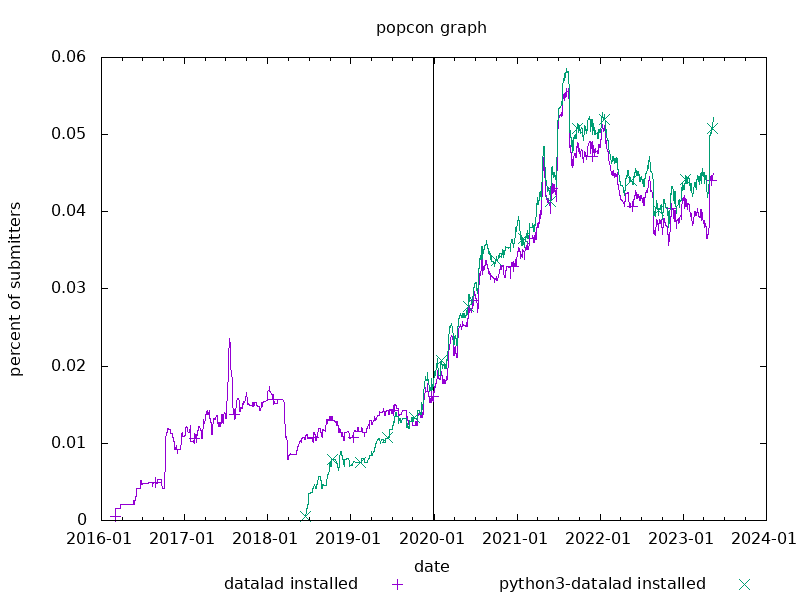
\includegraphics[width=\textwidth]{popcon-datalad.png}
	\caption{d}
	\label{fig:popcon}
\end{figure}

\pagebreak

